\documentclass{article}

\usepackage{biblatex}
\addbibresource{bib.bib}

\usepackage{graphicx}
\graphicspath{ {./images/} }

\title{Brain Image-Derived Phenotypes Regression Using Convolutional Neural Network}

\author{Bramantyo Ibrahim Supriyatno}

\date{April 2022}

\begin{document}
    \maketitle
    \begin{abstract}
        The use of convolutional neural networks (CNN) for computer vision problems has been significantly successful. 
        However, there is still a debate whether a complex non-linear model can outperform linear models for brain imaging data. 
        Knowing how each component of CNN affects its performance would be beneficial to addressing this debate. 
        In this project, we examine how each component of CNN contributes to the overall performance of the model in predicting brain image-derived phenotypes(IDPs). 
        We found that kernel size, strides number, and deeper network have profound effects on the performance, especially in gray-white contrast and mean thickness-related phenotypes.
    \end{abstract}
    
    \section*{Introduction}
    The convolutional neural network (CNN) has been proven very successful for many computer vision applications. 
    AlexNet\cite{alexnet} successfully reached state-of-the-art performance for image classification tasks on the ImageNet dataset. 
    Since then, the popularity of CNN has been rapidly growing.
    
    The use of CNN in brain imaging data has been studied likewise. 
    Wen\cite{wen} reported that three-dimensional structural magnetic resonance image (sMRI) CNN performs quite well for detecting Alzheimer's disease. 
    However, he also reported that the CNN model did not perform better than the support vector machine (SVM) model. 
    Peng\cite{peng} also studied the use of CNN on predicting age. He proposed a shallow and straightforward CNN model that achieved a good result. 
    Schulz\cite{schulz} studied the influence of model complexity and sample size on age prediction. 
    He demonstrated that deep networks did not achieve better results compared to standard machine learning algorithms. 
    However, a study by Abrol\cite{abrol} reported the contrary. 
    He argued that complicated features could be extracted by the presence of nonlinearity in the deep learning algorithm  
    although the CNN model that he used was slightly different from Peng and Schulz. 
        
    The architectural design differences used in the previous works prohibit an impartial comparison. 
    Therefore, there is a need to systematically study how each component in CNN affected its performance. 
    The effect of kernel size, strides number, number of layers, pooling types, and normalization methods are among the hyperparameters that should be studied.
    
    The effect of design choices of CNN for non brain images has been well-studied. 
    Smith\cite{smith} presented a guideline for designing CNN. 
    The guidelines recommended using pyramidal structure, downsampling between blocks, and max-pooling. 
    Lathuiliere\cite{lath} specifically studied the effect on regression tasks. 
    He suggested modifying the last fully connected layer before the output when using state-of-the-art (SOTA) architectures for different applications.

    Measuring performance only on a one-dimensional prediction task would constrain the CNN to only exploit features that are significant for the task. 
    This would force the algorithm to extract complex features and hinder its ability to distill more universal features. 
    Therefore predicting image-derived phenotypes (IDPs) would be more suitable for this study. 
    IDPs are phenotypes related to volumes, areas, thickness, gray-white contrast, and intensities in a certain part or region of the brain. 
    These phenotypes can be potential biomarkers relating to certain brain conditions. 

    \section*{Method}
    \begin{figure}[h]
        \centering
        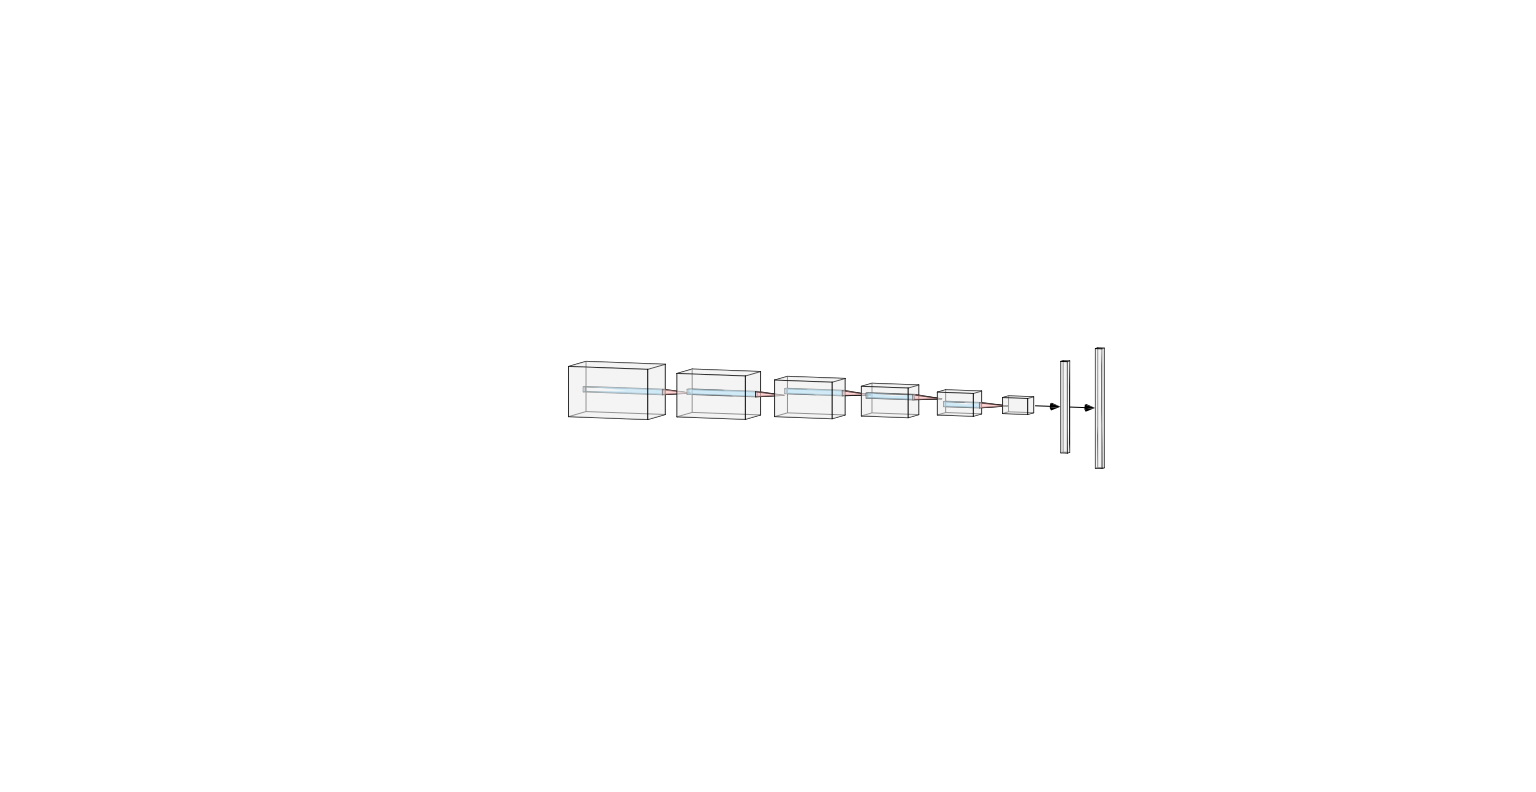
\includegraphics[scale=0.8]{nn}
        \centering
        \caption{
            Tensor view of modified version of simple-fully connected network with corresponding filter number for each block. This model was used as the baseline for the entire study}
        \label{fig:sfcn}
    \end{figure}
    \begin{table*}[h!]
        \begin{tabular}{||l c c c c||}
            \hline
            Model & MSE & Avg R2 & Num. Parameters & Num. Epochs \\
            \hline\hline
            vanilla & 0.84 & 0.19 & 3,044,301 & 18 \\
            \hline
            pyramid & 0.76 & 0.26 & 1,707,405 & 30 \\
            \hline
            avg pooling & 1.08 & -0.05 & 1,707,405 & 8 \\
            \hline
            strides pooling (size: 2) & 0.76 & 0.27 & 1,707,405 & 38 \\
            \hline
            strides pooling (size: 3) & 0.75 & 0.27 & 855,437 & 27 \\
            \hline
            kernel size: 2 & 0.75 & 0.27 & 811,821 & 25 \\
            \hline
            kernel size: 4 & 0.79 & 0.23 & 3,451,437 & 39 \\
            \hline
            downsampled & 0.71 & 0.31 & 1,707,405 & 26 \\
            \hline
            deeper & 0.68 & 0.34 & 1,720,877 & 31 \\
            \hline
            group norm: 8 & 0.78 & 0.25 & 1,705,805 & 56 \\
            \hline
            group norm: 16 & 0.80 & 0.23 & 1,705,805 & 43 \\
            \hline
            group norm ws: 8 & 0.74 & 0.29 & 1,705,805 & 49 \\
            \hline
            group norm ws: 16 & 0.80 & 0.23 & 1,705,805 & 44 \\ 
            \hline
            max global pooling & 0.65 & 0.37 & 1,707,405 & 38 \\
            \hline
            deeper max pool & 0.64 & 0.38 & 1,720,877 & 35 \\
            \hline
        \end{tabular}
        \caption{Mean-squared errors and average R2 scores for all models in this report}
        \label{table:1}
    \end{table*}
    CNN was initially proposed by LeCun\cite{lecun} in his groundbreaking paper. 
    The algorithm combines kernel convolution and gradient-based learning which updates the kernel weights. 
    The kernel convolution method reduces the number of parameters. 
    The use of backpropagation allows kernels to extract similar patterns across datasets. 
    These properties make the algorithm suitable for many computer vision problems such as optical character and object recognition.

    Modern CNN block comprises a convolutional layer, activation function, pooling layer, and normalization layer. 
    In the convolutional layer, parameter kernel size determines how big the kernel patch will be. 
    A bigger kernel size would allow more complex patterns in trade of an increasing number of parameters. 
    Strides number determine how much overlapping region each convolution will share. 
    A larger stride number will reduce overlap, although it will eventually result in loss of information. 
    Strides number also determines the output size of the convolution. 
    For example, strides number of 2 will halve the output size.

    A pooling layer often follows convolutional layer. 
    The purpose of the pooling layer is to select or combine the convolution output while reducing its size. 
    Downsampling can also be done by setting a proper strides number, despite algorithmically different. 
    The most common type of pooling is maximum pooling which picks the maximal value. 
    Another type of pooling is average pooling which takes the average value of the area.

    Afterwards, normalization layer is sometimes applied. Batch normalization normalizes the output value across the batch. 
    It also mitigates the effect of distribution shift across different input batches during training. 
    Batch normalization also acts as a regularizer.   
    However, batch normalization requires a large number of inputs per batch. 
    This can be a technical difficulty when having structural-MRI data. 
    The alternatives for smaller batch sizes are group standardization and weight normalization.

    This experiment studied how the hyperparameters affected the CNN's performance. 
    We chose a modified simple-fully connected network (SFCN) (Figure \ref{fig:sfcn}) as the baseline. 
    Hyperparameter modifications were applied then on this model. 
    Pairs of S-MRIs and IDPs values were used to train the network. 
    The S-MRIs are three-dimensional image data with a size of 190x210x190. 
    Preprocessing steps, such as standardization and cropping, were applied to keep the global mean to zero and throw out zero-valued voxels. 
    The network output was a vector of the size of the IDPs. 
    In this experiment, we picked 1421 IDPS values which did not have skewed distribution. 
    These values were also transformed by quantile transform with the number of quantiles 1000 following a normal distribution.

    This experiment used S-MRI data from UKBioBanks. 
    The dataset contained 10320 images which split into 60\% of the training set, 20\% of the validation set, and the remaining for the test set. 
    For every epoch, the program would take the mean-squared error (MSE) of validation set. 
    When there was no improvement for eight epochs, the training would stop. 
    When the training session stopped, the weights correspond to the lowest validation set's MSE would be kept.

    The experiments were conducted in a GPU cluster with 8 GTX 1080 ti totaling almost 100 gigabytes of GPU memory. 
    In general, training on 3D S-MRI data was exhaustive in terms of memory. 
    There was also a possibility of a bottleneck in data loading. 
    Therefore, data loading was performed by the CPU, while feedforwards and back-propagations were done by the GPU. 
    This experiment used Keras and TensorFlow in python.
    \section*{Results}
    
    \subsection*{Architectural Modification}
    \begin{figure}[h]
        \centering
        \includegraphics[scale=0.4]{vanillapyr}
        \centering
        \caption{
            Vanilla SFCN versus pyramidal SFCN. 
            Pyramidal structure improved all phenotypes prediction.}
        \label{fig:vanillapyr}
    \end{figure}
    The original SFCN has a bottleneck structure that limits the number of features to only 64 (Figure \ref{fig:sfcn}). 
    We then modified the number of filters so that the network has a pyramidal structure, as suggested by Smith\cite*[]{smith}. 
    We swapped the number of filters at the fourth and sixth convolutional blocks, so that we have this structure (32-64-64-128-256-256-1421). 
    This modification also reduced the number of parameters to almost half due to smaller filter numbers at the fourth convolutional block.

    The pyramidal model outperformed vanilla SFCN in all phenotype groups, as shown in figure \ref{fig:vanillapyr}. 
    The model also showed significant improvement in gray-white matter contrast (GWC), mean thickness, and mean intensity. 
    This improvement could be explained by the number of extracted features just before the last 1x1x1 convolutional layer. 
    The purpose of the bottleneck structure in the original model was for age prediction, in which the size of the final output vector is smaller than the number of extracted features. 
    Therefore bottleneck structure tends to be not suitable for IDP prediction.

    \subsection*{Kernel Size}
    
    \begin{figure}[h]
        \centering
        \includegraphics[scale=0.4]{kernsizes}
        \centering
        \caption{
            SFCN with different kernel sizes. 
            Gray-white matter contrast and mean thickness phenotypes were predicted better by smaller kernel.}
        \label{fig:kernsizes}
    \end{figure}

    Previous results in structural modification hinted at the idea that smaller number of parameters performed better. 
    SFCN has five convolutional layers that use 3x3x3 convolutional kernels. 
    These kernels can be resized and consequently reduce or increase the number of parameters. 

    Kernel size 2x2x2 reduced the number of parameters by half (table \ref{table:1}). 
    It also improved the R2 score for gray-white matter contrast and mean thickness, although there was a slight decrease in volume and area-related phenotypes (figure \ref{fig:kernsizes}). 
    Conversely, a bigger kernel size harmed almost all phenotypes despite a staggering increase in parameters.

    The results also indicated that the amount of overlapping receptive fields seemed to be important. 
    The smaller overlap caused by the smaller kernel improved the R2 score for gray-white matter contrast and thickness. 
    On the other hand, The larger kernel would increase the number of voxels shared by many filters. 
    As an example, the kernel size 4x4x4 will share 63 voxels. 
    It means that each filter would receive similar data. 
    Thus it becomes hard to extract distinct features from the data.


    \subsection*{Downsampling and Pooling Method}
    
    \begin{figure}[h]
        \centering
        \includegraphics[scale=0.4]{poolstrides}
        \centering
        \caption{
            Different downsampling methods and strides numbers on SFCN. 
            Methods with less overlap seemed to perform better especially on gray-white matter and thickness phenotypes.}
        \label{fig:poolstrides}
    \end{figure}

    Downsampling can be done by adding a pooling layer or setting up a larger strides number on the convolution layer. 
    The amount of downsampling in the pooling layer is controlled by the pooling size. Furthermore, type of pooling layer determine how the downsampling is performed.   

    Average pooling did not accomplish well and did not seem to learn well (figure \ref{fig:poolstrides}). 
    Average pooling would weigh all convolutional output by the same value, thus increasing the chance of significant features being treated equally. 
    Although it could be compensated by increasing the corresponding weight on the convolutional kernel, it would take more time and could need different learning rate scheduling to train the model.

    On the other hand, max-pooling selects the maximum value and only back-propagates the weight corresponding to the value. 
    Since the training data were registered, locations of one particular brain area were not largely different image by image. 
    This property allowed max pooling to extract important features more accurately and faster. 
    Additionally, maximum pooling mitigated the overlapping effect.

    Downsampling using strides performed on par with the baseline despite less computation. 
    Strides number two predicted gray-white matter contrast better than the baseline. 
    Strides number three also performed slightly better even though there were significant reductions in the number of parameters due to a bigger downsampling scale. 
    The result confirms that gray-white matter contrast predictions were sensitive to the amount of overlapping.

    Notice that strides number three also reduced the size of the voxels when entering the global pooling layer. 
    A smaller global pooling size would possibly reduce the overlapping effect observed in the previous experiment on kernel size and pooling types

    \subsection*{Global Pooling Size and Type}
    
    \begin{figure}[h]
        \centering
        \includegraphics[scale=0.4]{sizeatglopol}
        \centering
        \caption{
            Global pooling sizes and type on SFCN. 
            Smaller sizes at the global pooling were preffered although maximum pooling outperformed average pooling.}
        \label{fig:glopolsizetype}
    \end{figure}
    
    Previous experiments on downsampling methods denoted that a smaller number of voxels when entering a global pooling layer was beneficial. 
    Global pooling size can be reduced by downsampling the input and increasing the depth of the network. 
    Additionally, choosing maximum pooling instead of average pooling reduces the size to one in a non-linear manner.

    In general, both downsampling input data and increasing the depth of the network elevated the R2 scores in almost all phenotypes (figure \ref{fig:glopolsizetype}). 
    Changing the pooling type to maximum pooling improved the prediction further. 
    This indicated that there was some unnecessary information at the global pooling that can be omitted.
    Average global pooling would weight the data uniformly thus it barely omitted the unnecessary information. 
    Maximum pooling would choose the biggest value thus in a way it would only selected the significant information. 
    Furthermore, improvement by downsampling the input indicated that these unnecessary information could be originated from the image data.
        
    \subsection*{Normalization Method}
   
    \begin{figure}[h]
        \centering
        \includegraphics[scale=0.4]{normtypes}
        \centering
        \caption{
            Different normalization methods on SFCN. 
            Group normalization with size of 8 were a good alternative to batch normalization}
        \label{fig:normtypes}
    \end{figure}

    One particular problem when working with huge structural MRI data is the limitation of GPU memory. 
    This affects the number of batches when feed forwarding and has a direct implication when choosing the normalization method. 
    Batch normalization with size 8 seems to be the best choice when having adequate memory. 
    However, group normalization with weight standardization with batch size 8, which can be used when having limited memory, has similar performance despite a longer training time (figure \ref{fig:normtypes}). 
    Notice that bigger groups did not always deliver a better performance. 
    Additionally, group normalization seemed to increase performance for gray-white matter contrast as well as mean thickness.

   
    \section*{Conclussions and Summary}
    When repurposing SOTA implementation, it is recommended to start modifying the deepest layer first. 
    Changing the number of extracted features seems to be beneficial especially when the target outputs are bigger than the number of extracted features. 
    In addition, changing the global pooling type could be necessary when having large dimensional data.

    Furthermore, deeper networks perform significantly better compared to the shallower ones. 
    A deeper network minimizes the size of the volumes when entering the global pooling layer which is also found to be beneficial. 
    However, increasing the number of parameters could lengthen the training time.
    
    Design choices also affect the model performance on certain phenotypes. 
    Minimizing overlap by increasing strides value or using a smaller kernel size seems to be beneficial for predicting gray-white matter contrast and mean thickness-related phenotypes.
    
    \printbibliography
\end{document}